
\section{Sistemas HAR}
\begin{frame}{Sistemas HAR}

\framesubtitle{Aplicaciones de Contexto}

\setbeamercovered{transparent}
\begin{itemize}
\item Aplicaciones cuyo medio de interacci�n es adem�s el contexto.
\end{itemize}

\pause{}
\begin{itemize}
\item El contexto es el estado acerca de la informaci�n
\begin{itemize}
\item f�sica
\item emocional
\item social, entre otros
\end{itemize}
\end{itemize}

\pause{}
\begin{itemize}
\item La computaci�n m�vil y ubicua es sin�nimo de dinamismo en el contexto
\end{itemize}

\pause{}
\begin{itemize}
\item Tipos de contexto comunes en computaci�n m�vil son 
\begin{itemize}
\item la ubicaci�n, 
\item la identidad, 
\item la actividad 
\item y el tiempo
\end{itemize}
\end{itemize}
\end{frame}
%
\begin{frame}[shrink]{Sistemas HAR}

\framesubtitle{Actividades Humanas}

\setbeamercovered{transparent}
\begin{block}{Actividades Simples}
Acciones simples peri�dicas de larga duraci�n.
\end{block}
\begin{center}
\uncover<2->{\begin{center}
\begin{tabular}{|c|>{\raggedright}p{5cm}|}
\hline 
Ambulatorias & Caminar, correr, sentarse, pararse, quieto, acostarse, subir y descender
escaleras.\tabularnewline
\hline 
Transporte & En bus, bicicleta y conducir.\tabularnewline
\hline 
\end{tabular}
\par\end{center}}
\par\end{center}
\begin{block}{Actividades Complejas}
Acciones cortas o peri�dicas no comunes.
\end{block}
\begin{center}
\uncover<3->{\begin{center}
\begin{tabular}{|c|>{\raggedright}p{5cm}|}
\hline 
Cotidianas & Comer, beber, mirar TV, leer, cepillarse los dientes, entre otros.\tabularnewline
\hline 
Gimnasio & Alzar pesas, ejercicio aer�bico, bicicleta est�tica.\tabularnewline
\hline 
Militares & Arrastrarse, en cuclillas.\tabularnewline
\hline 
\end{tabular}
\par\end{center}}
\par\end{center}

\end{frame}
%
\begin{frame}{Sistemas HAR}

\framesubtitle{Objetivos del sistema}

\setbeamercovered{transparent}
\begin{itemize}[<+->]
\item Proveer un m�dulo base para el desarrollo de aplicaciones de contexto. 
\item Reconocer varias actividades realizadas rutinariamente de diferentes
maneras, por diferentes usuarios y en diferentes condiciones contextuales.
\end{itemize}
\begin{center}
\visible<2>{\begin{center}
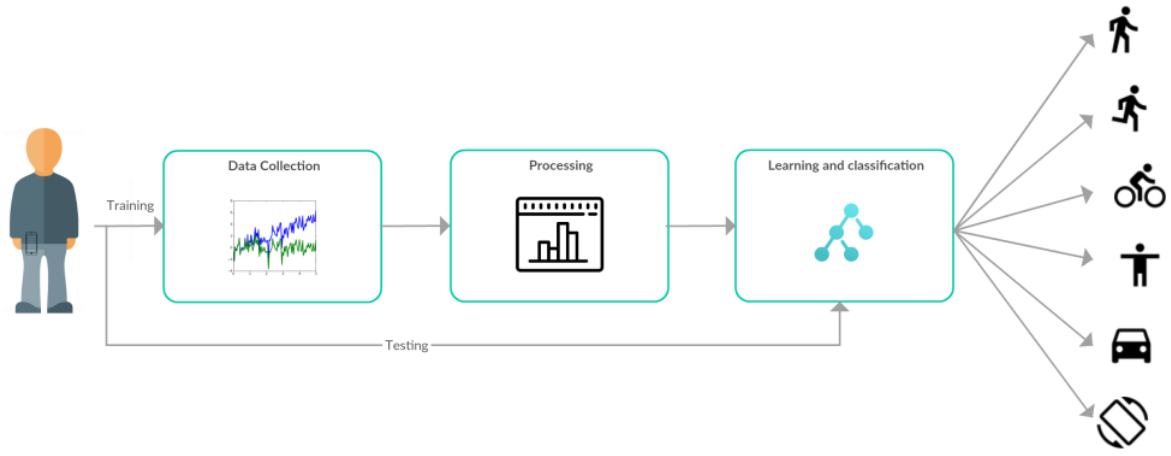
\includegraphics[width=0.8\textwidth]{../capitulo-2/graphics/harsystem2}
\par\end{center}}
\par\end{center}

\end{frame}
%
\begin{frame}{Sistemas HAR}

\framesubtitle{Dise�o del sistema}

\setbeamercovered{transparent}
\begin{itemize}
\item Arquitectura basada en aplicaciones de aprendizaje autom�tico (\emph{Machine Learning},
ML).
\end{itemize}

\pause{}
\begin{itemize}
\item Componentes principales
\begin{itemize}
\item un \structure{recolector} de medidas 
\item un \structure{procesador} de muestras 
\item un \structure{clasificador} de actividades
\end{itemize}
\end{itemize}

\pause{}
\begin{itemize}
\item Metodolog�a operativa
\begin{itemize}
\item Aprendizaje fuera de linea (\emph{off-line})
\item Clasificaci�n en linea (\emph{on-line})
\end{itemize}
\end{itemize}
\begin{center}
\visible<2->{\begin{center}
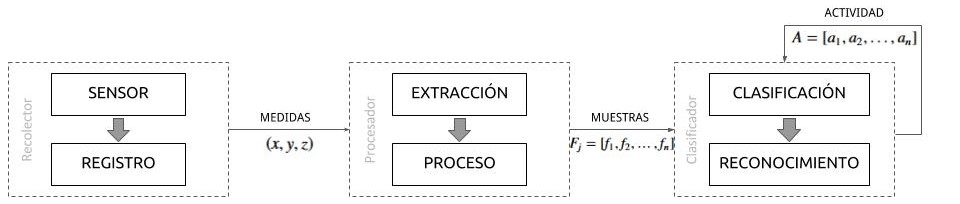
\includegraphics[width=0.8\textwidth]{../capitulo-4/graphics/diagrama_4_1}
\par\end{center}}
\par\end{center}

\end{frame}
%
\begin{frame}{Sistemas HAR}

\framesubtitle{Componentes}

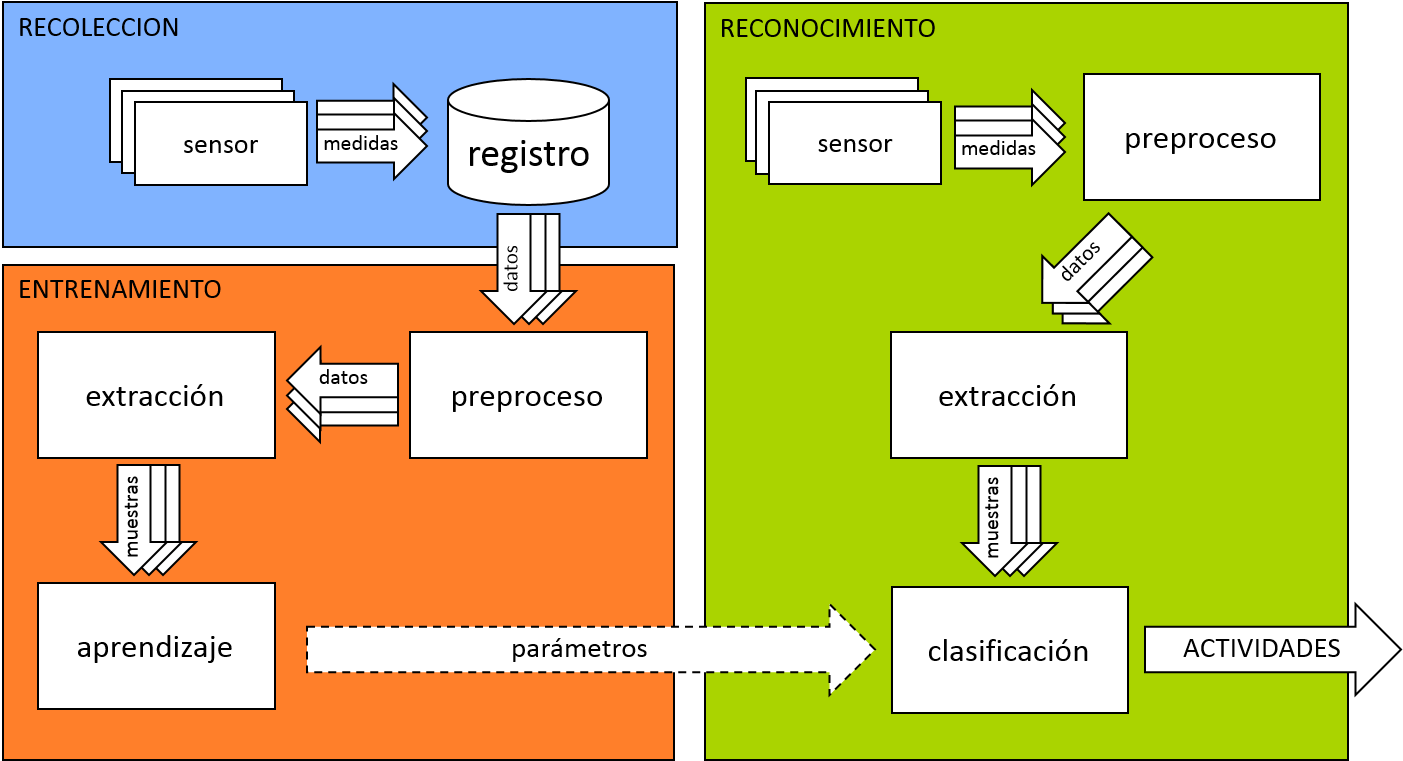
\includegraphics[width=1\columnwidth]{propuesta/graphics/harsystem}
\end{frame}

